\section{Analysis}\label{sec:analysis}

In this section we examine the macro-topological structure of the
unfiltered and filtered token graphs including degree distributions,
connected component structure, and cyclic structure.  We also examine
the micro-topological structure of some individual tokens.  We
visualise the composition of tokens and identify their direct and
transitive dependencies.

\begin{table}
  \centering
  \caption{Each edge in a token graph represents a set of tokenising
    meta-events.  The top five most significant edges in terms of the
    number of tokenising meta-events they contain are shown.  The
    results are the same for both the unfiltered and filtered token
    graphs, i.e., the same five edges are present in
    both.}\label{tab:most-significant-edges}
  \begin{tabular}{|c|c|r|}
    \hline

    Source Token & Target Token & \begin{tabular}{@{}c@{}}\#
      Tokenising\\Meta-Events\end{tabular}\\

    \hline

    \texttt{SHIB}~(\texttt{0x95ad61}) &
    \texttt{xSHIB}~(\texttt{0xb4a812}) & \num{402186}\\

    \texttt{BONE}~(\texttt{0x981303}) &
    \texttt{tBONE}~(\texttt{0xf7a038}) & \num{203734}\\

    \texttt{SUSHI}~(\texttt{0x6b3595}) &
    \texttt{xSUSHI}~(\texttt{0x879824}) & \num{120221}\\

    \texttt{LEASH}~(\texttt{0x27c70c}) &
    \texttt{xLEASH}~(\texttt{0xa57d31}) & \num{75180}\\

    \texttt{USDC}~(\texttt{0xa0b869}) &
    \texttt{aUSDC}~(\texttt{0xbcca60}) & \num{69373}\\

    \hline
  \end{tabular}
\end{table}

We note that each edge in a token graph represents a set of tokenising
meta-events.  Before examining the structure of the graphs, we can
identify the most significant edges in terms of the number of
tokenising meta-events they contain.
Table~\ref{tab:most-significant-edges} shows the results for both the
unfiltered and filtered token graphs.  Three of the five edges
represent the staking of memecoins
(\texttt{SHIB}~$\rightarrow$~\texttt{xSHIB},
\texttt{BONE}~$\rightarrow$~\texttt{tBONE}, and
\texttt{LEASH}~$\rightarrow$~\texttt{xLEASH}), one represents the
staking of a governance token for a decentralised exchange
(\texttt{SUSHI}~$\rightarrow$~\texttt{xSUSHI}), and one represents the
supply of a stablecoin to a decentralised lending market
(\texttt{USDC}~$\rightarrow$~\texttt{aUSDC}).  Of course, we could
also measure the significance of a edge based on, say, the volume of
tokens transacted, the present USD value of the locked tokens, etc.

\subsection{Degree Distributions}\label{sec:analysis-degree-distribution}

\begin{figure}
  \centerline{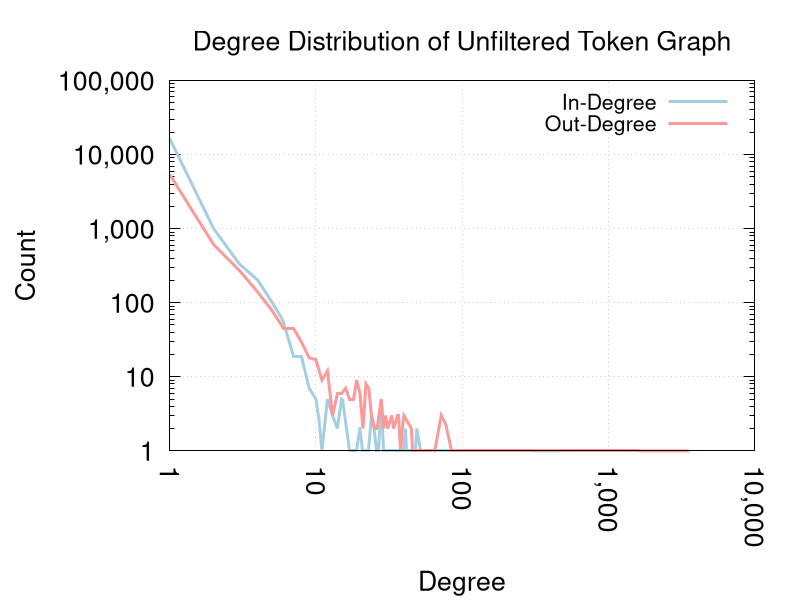
\includegraphics[width=\columnwidth]{img/degree-distributions/unfiltered-token-graph-degrees.png}}
  \caption{The in- and out-degree distributions of the unfiltered
    token graph show an inverse relationship between the degree of a
    vertex and the number of vertices with that degree in the graph.
    There are a small number of vertices with high degree and a large
    number of vertices with low
    degree.}\label{fig:unfiltered-token-graph-degrees}
\end{figure}

\begin{figure}
  \centerline{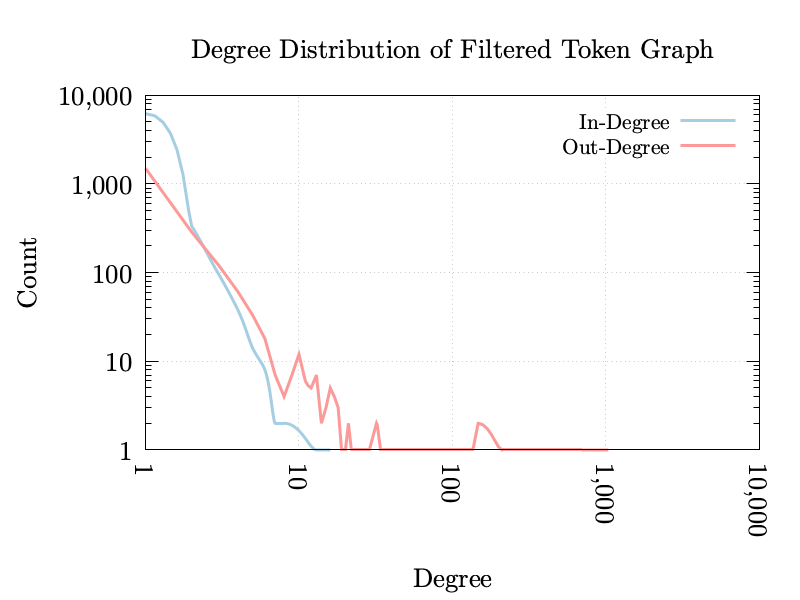
\includegraphics[width=\columnwidth]{img/degree-distributions/filtered-token-graph-degrees.png}}
  \caption{The in- and out-degree distributions of the filtered token
    graph show a similar inverse relationship as in
    Fig.~\ref{fig:unfiltered-token-graph-degrees}.}\label{fig:filtered-token-graph-degrees}
\end{figure}

\begin{table}
  \centering
  \caption{The top five vertices (tokens) in the unfiltered and
    filtered token graphs by in-degree and
    out-degree.}\label{tab:highest-in-out-degrees}
  \begin{tabular}{|c|c|r|c|r|}
    \hline

    & \multicolumn{2}{c|}{Top Five by In-Degree} &
    \multicolumn{2}{c|}{Top Five by Out-Degree}\\

    \cline{2-5}

    & Token & Deg. & Token & Deg.\\

    \hline

    \multirow{5}{0pt}{\rotatebox{90}{Unfiltered}}

    & \texttt{CHI}~(\texttt{0x000000}\footnote{The contract address
    for \texttt{CHI} is
    \texttt{0x0000000000004946c0e9f43f4dee607b0ef1fa1c}.}) & \num{471}
    & \texttt{USDC}~(\texttt{0xa0b869}) & \num{3587}\\

    & \texttt{USDP}~(\texttt{0x145668}) & \num{117} &
      \texttt{DAI}~(\texttt{0x6b1754}) & \num{1923}\\

    & \texttt{aUSDC}~(\texttt{0xbcca60}) & \num{84} &
      \texttt{USDT}~(\texttt{0xdac17f}) & \num{1175}\\

    & \texttt{aWETH}~(\texttt{0x030ba8}) & \num{63} &
      \texttt{WETH}~(\texttt{0xc02aaa}) & \num{951}\\

    & \texttt{aDAI}~(\texttt{0x028171}) & \num{54} &
      \texttt{sUSD}~(\texttt{0x57ab1e}) & \num{548}\\

    \hline

    \multirow{5}{0pt}{\rotatebox{90}{Filtered}}

    & \texttt{XDP2}~(\texttt{0xe68c1d}) & \num{16} &
    \texttt{USDC}~(\texttt{0xa0b869}) & \num{1037}\\

    & \texttt{XDP1}~(\texttt{0x134fc6}) & \num{15} &
    \texttt{DAI}~(\texttt{0x6b1754}) & \num{752}\\

    & \texttt{cyUSD}~(\texttt{0x1d0914}) & \num{14} &
    \texttt{USDT}~(\texttt{0xdac17f}) & \num{396}\\

    & \texttt{iDOL}~(\texttt{0x7591a3}) & \num{13} &
    \texttt{WETH}~(\texttt{0xc02aaa}) & \num{281}\\

    & \texttt{agEUR}~(\texttt{0x1a7e4e}) & \num{8} &
    \texttt{WBTC}~(\texttt{0x2260fa}) & \num{211}\\

    \hline
  \end{tabular}
\end{table}

The in- and out-degree distributions of the unfiltered and filtered
token graphs show an inverse relationship between the degree of a
vertex and the number of vertices with that degree in the graph (see
Fig.~\ref{fig:unfiltered-token-graph-degrees} and
Fig.~\ref{fig:filtered-token-graph-degrees}).
Table~\ref{tab:highest-in-out-degrees} shows the top five vertices in
the unfiltered and filtered token graphs by in-degree and out-degree.
The out-degree entries are easy to explain: they are the tokens that
are deposited with contracts in order to mint many other types of
tokens.  They include stablecoins (\texttt{USDC}, \texttt{DAI},
\texttt{USDT} and \texttt{sUSD}), wrapped ether (\texttt{WETH}), and
wrapped bitcoin (\texttt{WBTC}).  The in-degree entries are more
complex and have multiple explanations.  For example,
\texttt{CHI}~\cite{1inch-20} is a gas token created by 1inch, a
decentralised exchange aggregator, that is burned to obtain a
reduction in transaction fees; in some transactions the burning of
\texttt{CHI} is combined with the withdrawal of another token.  This
is a false positive generated by our heuristic since \texttt{CHI} does
not tokenise a token.  The remaining in-degree entries in the
unfiltered category are due to token swaps performed during a deposit.
For example, \texttt{aDAI}~\cite{aave-xx} is a yield-bearing token
issued by AAVE, a decentralised lending market, in exchange for the
stablecoin \texttt{DAI}.  However, in some transactions, other tokens
are supplied and swapped to \texttt{DAI}.  These are also false
positives since only \texttt{DAI} is tokenised by \texttt{aDAI}.  In
the filtered category, the in-degree entries are more reliable.  For
example, the \texttt{iDOL} token is minted when a user deposits
various forms of the \texttt{SBT} token (e.g., \texttt{SBT09180200},
\texttt{SBT09250200}, etc.) according to the Lien
Protocol~\cite{lien-20}.  Similarly, the \texttt{agEUR} token is a
stablecoin by the Angle Protocol~\cite{angle-xx} that accepts a
variety of tokens as collateral.

\begin{figure}
  \centerline{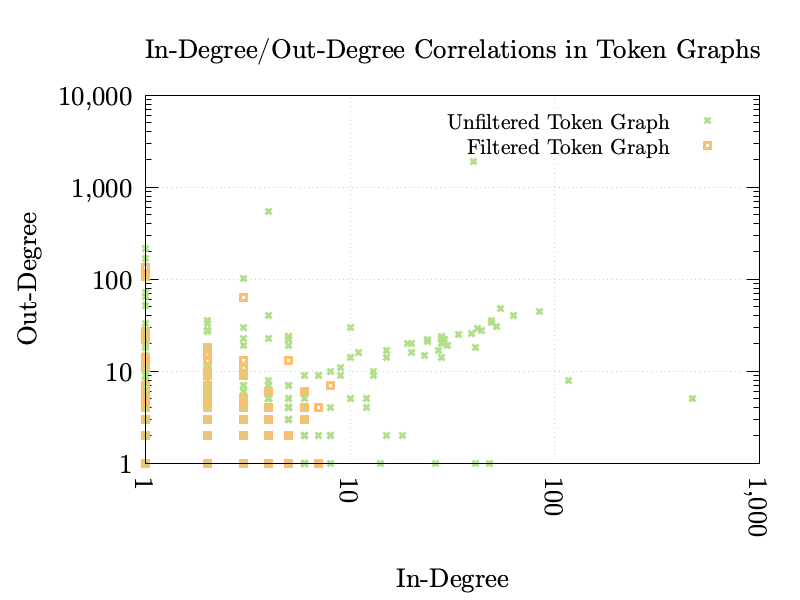
\includegraphics[width=\columnwidth]{img/degree-distributions/token-graph-in-out-degrees.png}}
  \caption{In the unfiltered and filtered token graphs, we can
    identify vertices with both high in-degree and high
    out-degree.}\label{fig:token-graph-in-out-degrees}
\end{figure}

Figure~\ref{fig:token-graph-in-out-degrees} plots in-degrees against
out-degrees in the unfiltered and filtered token graphs.  The tokens
whose corresponding vertices have both high in-degree and high
out-degree are tokens that tokenise many other tokens, and are
themselves tokenised by many other tokens.  Examples include
\texttt{mUSD}, a stablecoin issued by the mStable
protocol~\cite{mstable-xx} and the \texttt{agEUR} token.  This makes
intuitive sense as stablecoins can be minted from various forms of
collateral, and stablecoins can be used as collateral to mint other
tokens.

\subsection{Connected Component Structure}\label{sec:analysis-component-structure}

The unfiltered graph has \num{4082} weakly connected components.  A
giant component contains \num{13794} vertices ($\sim$\num{58}\%) and
\num{17711} edges ($\sim$\num{75}\%).  \num{3336} components
($\sim$\num{82}\% of the total) contain two connected vertices.  These
vertices correspond to pairs of tokens where at least one tokenises
the other, but neither tokenises, or is tokenised by, a third.
Interestingly, none of the tokens represented by vertices in these
components have a non-zero market capitalisation according to
CoinGecko or are traded in a liquidity pool according to DEX Screener.
Their lack of popularity reflects their isolation in the token graph.

\begin{figure}
  \centerline{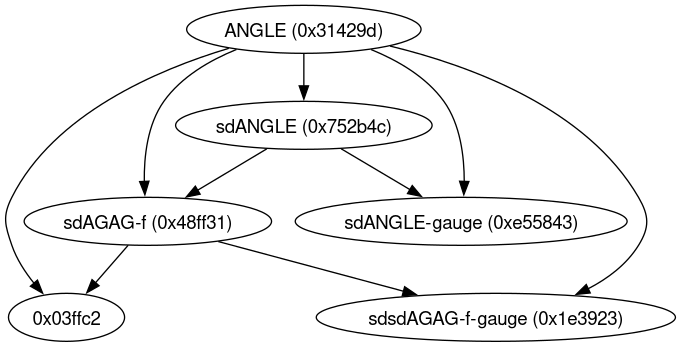
\includegraphics[width=\columnwidth]{img/medium-components/angle-protocol.png}}
  \caption{The unfiltered token graph contains a weakly connected
    component whose vertices correspond to tokens related to the Angle
    Protocol and Stake DAO.}\label{fig:angle-protocol}
\end{figure}

There are \num{418} components, other than the giant component, with
more than two connected vertices.  Figure~\ref{fig:angle-protocol} is
an example from this set.  It shows the tokenising relationships
between tokens related to the Angle Protocol~\cite{angle-xx} and Stake
DAO~\cite{stake-dao-xx}.  Stake DAO implements investment strategies
based on other decentralised protocols.  Their ``Liquid Lockers''
produce liquidity, voting power, and yield from lockable tokens.
\texttt{ANGLE} is Angle's governance token.  It can be deposited with
Stake DAO to mint \texttt{sdANGLE}.  It is not possible to burn
\texttt{sdANGLE} and withdraw \texttt{ANGLE}: the edge between those
vertices represents a one-way operation and is present in the
unfiltered token graph but not in the filtered version. \texttt{ANGLE}
and \texttt{sdANGLE} can be deposited in a gauge (liquidity pool) to
mint \texttt{sdANGLE-gauge}.  We can use this visualisation to
identify the direct and transitive dependencies of tokenising tokens
such as \texttt{sdANGLE} and \texttt{sdANGLE-gauge}.  Many of the
other components in the set produce similar insights that relate to
other tokens and protocols.

\begin{figure*}
  \centerline{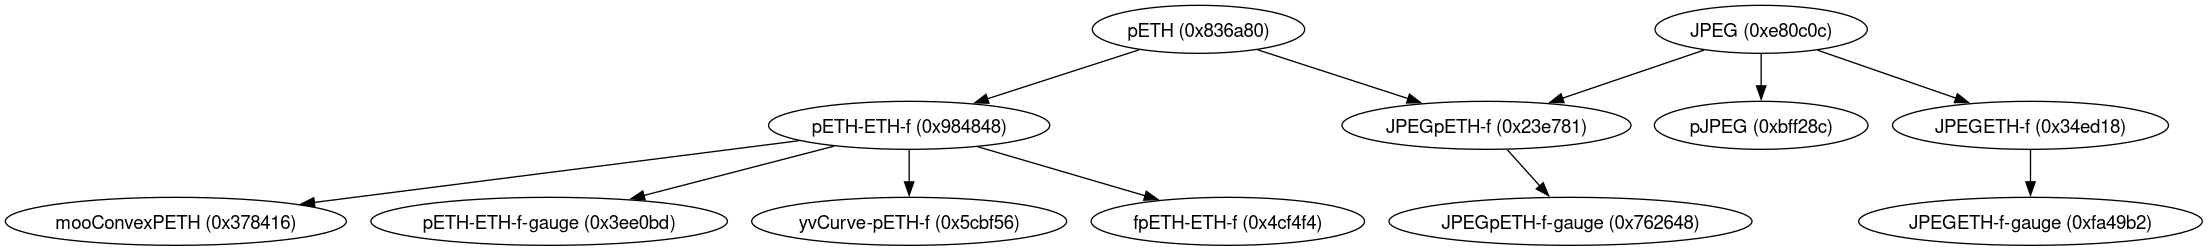
\includegraphics[width=\textwidth]{img/medium-components/jpegd-protocol.png}}
  \caption{The filtered token graph contains a weakly connected
    component whose vertices correspond to tokens related to the
    JPEG'd Protocol.}\label{fig:jpegd-protocol}
\end{figure*}

The filtered graph has \num{1491} weakly connected components.  A
giant component contains \num{4648} vertices ($\sim$\num{55}\%) and
\num{5247} edges ($\sim$\num{70}\%).  \num{1162} components
($\sim$\num{78}\% of the total) contain two connected vertices.  There
are \num{196} components, other than the giant component, with more
than two connected vertices.  Figure~\ref{fig:jpegd-protocol} is an
example from this set that relates to the JPEG'd
Protocol~\cite{jpegd-xx}.  JPEG'd is a decentralised lending market
where users can supply non-fungible-tokens (NFTs) as collateral and
obtain loans in \texttt{pETH}, a synthetic token that tracks the price
of ether. \texttt{JPEG} is the protocol's governance token.  The
figure shows the various ways in which \texttt{pETH} and \texttt{JPEG}
can be tokenised by liquidity pools such as Curve's \texttt{pETH/WETH}
pool~\cite{curve-finance-xx}. Unlike the operations represented by
edges in Fig.~\ref{fig:angle-protocol}, all operations represented by
edges in Fig.~\ref{fig:jpegd-protocol} can be reversed by burning the
tokenising tokens and withdrawing the underlying.

Both the unfiltered and filtered graphs contain giant weakly connected
components.  Exploring such structures requires an interactive user
interface with navigational aids such as selection, panning, and
zooming.  As an illustrative example of the interesting structure in
the giant components, we identified the longest directed path in the
filtered token graph.  It comprises nine vertices and represents the
following sequence of tokens:

\begin{enumerate}
\item \texttt{renBTC}~(\texttt{0xeb4c27})
\item \texttt{sBTC}~(\texttt{0xfe18be})
\item \texttt{crvRenWSBTC}~(\texttt{0x075b1b})
\item \texttt{tbtc/sbtcCrv}~(\texttt{0x64eda5})
\item \texttt{btbtc/sbtcCrv}~(\texttt{0xb9d076})
\item \texttt{ibBTC}~(\texttt{0xc4e159})
\item \texttt{wibBTC}~(\texttt{0x8751d4})
\item \texttt{ibbtc/sbtcCRV-f}~(\texttt{0xfbdca6})
\item \texttt{bibbtc/sbtcCRV-f}~(\texttt{0xae96ff})
\end{enumerate}

\texttt{renBTC} can be deposited with a contract to mint
\texttt{sBTC}, \texttt{sBTC} can be deposited with a contract to mint
\texttt{crvRenWSBTC}, etc.  The reverse operations can also be
performed (withdraw \& burn).  The chain involves tokens from several
different protocols.  It is an example of ``composition in the wild''
--- groups of interacting smart contracts than span multiple
protocols.

\subsection{Cyclic Structure}\label{sec:analysis-cyclic-structure}
